%% ================================================================
%% Dissertação de Mestrado — UFPE / Departamento de Eletrônica e Sistemas
%% Autenticação na Camada Física com Tags Caóticas via Discriminador Neural
%% Autor: Thamires Tavares | Orientadores: D. Chaves, C. Pimentel
%%
%% Compilar:  pdflatex dissertacao.tex  (ou lualatex)
%% Nota: trocar \documentclass pelo template oficial UFPE quando disponível.
%% ================================================================
\documentclass[12pt,a4paper]{article}
\usepackage[brazil]{babel}
\usepackage[utf8]{inputenc}
\usepackage[T1]{fontenc}
\usepackage{amsmath}
\usepackage{amssymb}
\usepackage{graphicx}
\usepackage{booktabs}
\usepackage[margin=2.5cm]{geometry}
\usepackage{setspace}
\usepackage[colorlinks=true,linkcolor=blue,citecolor=blue,urlcolor=blue]{hyperref}
\usepackage{microtype}
\graphicspath{{figures/}}
\onehalfspacing
%% ================================================================

\begin{document}

\title{\textbf{Autenticação na Camada Física com Tags Caóticas\\via Discriminador Neural}\\[0.5em]
\large Ablação das Entradas e Núcleo Mínimo em Canal Rayleigh}

\author{Thamires Tavares\\[0.4em]
\small Orientadores: Prof.\ Daniel P.\ B.\ Chaves e Prof.\ Cecílio J.\ L.\ Pimentel\\
\small Departamento de Eletrônica e Sistemas --- UFPE, Recife\,--\,PE}

\date{\textit{Versão de trabalho} --- Julho de 2026}

\maketitle
\thispagestyle{empty}


\renewcommand{\abstractname}{Resumo}
\begin{abstract}
\noindent
Este trabalho propõe a aplicação de um discriminador neural orientado a dados (\textit{Data-Driven Detection Framework}, D3F) ao problema de autenticação na camada física com sequências caóticas em canais Rayleigh. A investigação parte de uma pergunta prática fundamental: qual representação de entrada é mais adequada para o discriminador neural --- o sinal residual bruto $\mathbf{z}_{eq}$, um vetor de características fisicamente motivadas, ou um subconjunto ainda menor?

O trabalho contribui em três frentes: (i)~\textbf{primeira aplicação do D3F} ao cenário de PLA com tags caóticas em canal Rayleigh, demonstrando que o framework é diretamente aplicável e eficaz; (ii)~\textbf{comparação de representações de entrada} --- mostrando que abordagens baseadas em sinal bruto ($\mathbf{z}_{eq}$) falham em baixo SNR por ausência de integração coerente implícita, enquanto características escalares fisicamente motivadas superam o correlador clássico em dez vezes a 0~dB; e (iii)~\textbf{estudo de ablação sistemático} que, partindo do correlador casado $|\tau|$ como estatística suficiente de Neyman-Pearson, identifica o núcleo mínimo de características necessário.

Os resultados do estudo de ablação --- com variantes V5\,($[|\tau|]$), V6\,($[|\tau|, \hat{h}]$), V7\,($[|\tau|, \hat{h}, \overline{\text{SNR}}]$), V8\,($[|\tau|, \hat{h}, E]$) e V1\,($[|\tau|, \hat{h}, \overline{\text{SNR}}, E]$) --- confirmarão se o par $[|\tau|, \hat{h}]$ é de fato mínimo e suficiente, ou se a energia instantânea $E$ traz ganho real.

\vspace{0.8em}
\noindent\textbf{Palavras-chave:} Autenticação na camada física, discriminador neural, D3F, 1D CNN, canal Rayleigh, ablação de características, sequências caóticas, CFAR, Neyman-Pearson.
\end{abstract}

\newpage
\tableofcontents
\newpage

\section{Introdução}

A autenticação de dispositivos em redes sem fio é um requisito de segurança cada vez mais crítico, especialmente com a expansão de sistemas IoT e 5G/6G~\cite{ref_xie}. Em cenários veiculares (\textit{Vehicle-to-Everything}, V2X)~\cite{ref_3gpp}, por exemplo, dispositivos precisam ser autenticados em dezenas de milissegundos enquanto se deslocam a alta velocidade — janela de tempo incompatível com protocolos de troca de chaves convencionais, que exigem múltiplas rodadas de troca de mensagens entre as partes~\cite{ref_raya}. Abordagens criptográficas tradicionais, implementadas nas camadas superiores da pilha de protocolos, pressupõem capacidade computacional e infraestrutura de gerenciamento de chaves incompatíveis com dispositivos de recursos limitados e com a escala de redes heterogêneas emergentes.

A autenticação na camada física (\textit{Physical Layer Authentication}, PLA) surge como solução complementar, explorando características do sinal transmitido — intrínsecas ao canal e difíceis de reproduzir por adversários sem acesso ao canal legítimo — sem exigir complexidade adicional no receptor. PLA divide-se em duas estratégias: (i) \textbf{PLA passiva}, que extrai características naturais do canal (desvanecimento, espalhamento de atraso) para verificar legitimidade~\cite{ref_poor}, e (ii) \textbf{PLA ativa}, que insere sequências de autenticação de baixa potência (tags) sob controle criptográfico do transmissor legítimo, garantindo que apenas receptores com a chave secreta compartilhada possam detectá-las~\cite{ref_joao}.

 \subsection{Definição do Problema}

Este trabalho foca em PLA ativa por inserção de sequências caóticas~\cite{ref_yu}. Geradas a partir de uma chave secreta compartilhada entre transmissor legítimo e receptor, essas sequências (tags) são detectáveis apenas por correlação com a referência conhecida, provendo sigilo intrínseco~\cite{ref_joao}. O problema é formulado como teste de hipótese binária: $H_0$ (ausência de tag legítima $\Rightarrow$ intruso) contra $H_1$ (tag presente $\Rightarrow$ transmissor autêntico).

Em canais com desvanecimento Rayleigh, essa discriminação torna-se crítica em baixo SNR: o ganho de canal varia de pacote a pacote, alterando a distribuição do correlator casado~\cite{ref_xie}, dificultando manter simultaneamente alta probabilidade de detecção $P_D$ e falso positivo reduzido. Sistemas práticos exigem probabilidades de falso positivo da ordem de $\alpha = 10^{-7}$ para aplicações veiculares em tempo real~\cite{ref_raya,ref_xie}, pois cada autenticação falsa negativa representa risco de segurança. A verificação direta dessa restrição por simulação Monte Carlo demandaria aproximadamente $1/\alpha \approx 10^7$ amostras sob $H_0$ por ponto de operação — tornando a avaliação computacionalmente proibitiva. A eficiência computacional é determinante em sistemas embarcados veiculares com restrições de latência e consumo energético.

\subsection{Solução proposta}

O obstáculo computacional é contornado pelo \textit{Data-Driven Detection Framework} (D3F)~\cite{ref_braca}, que constrói detectores de Neyman-Pearson ótimos a partir de dados, sem necessidade de conhecer explicitamente as distribuições de probabilidade das estatísticas de decisão. A estratégia repousa em dois pilares: (i)~treinar um classificador neural com entropia cruzada binária (BCE), que força escores de decisão calibrados; e (ii)~ajustar uma gaussiana aos escores sob $H_0$ em poucas amostras ($\sim 10^3$--$10^4$), permitindo extrapolação analítica do limiar $\tau^*(\alpha)$ via inversão da CDF gaussiana, sem simular $10^8$ amostras.

Como aplicação original, este trabalho propõe: (i)~D3F aplicado ao PLA com tags caóticas em Rayleigh, usando vetor $\mathbf{f} = [|\tau^i|, \hat{h}, \widehat{\text{SNR}}, E]$ fisicamente motivado por teoria de detecção; (ii)~comparação sistemática entre representações (características explícitas \textit{vs.} CNN 1D sobre sinal bruto); (iii)~ablação que identifica o par mínimo suficiente $[|\tau|, \hat{h}]$, com a feature $E$ emergindo como proxy empiricamente forte, porém menos fundamentada teoreticamente — resultado que motiva investigação da estrutura de informação no problema.

\section{Fundamentação Teórica}

\subsection{Modelo do Canal e Sinais}

Considera-se um cenário com transmissor legítimo (Alice), receptor (Bob) e atacante (Eve) em canal com desvanecimento plano e lento de Rayleigh~\cite{ref_poor}. No $i$-ésimo intervalo de sinalização, Alice transmite $\mathbf{x}^i = \rho_s \mathbf{s}^i + \rho_t \mathbf{t}^i$, onde $\mathbf{s}^i \in \{-1,+1\}^L$ é mensagem BPSK de $L$ símbolos e $\mathbf{t}^i$ é a tag caótica. Os parâmetros $\rho_s$ e $\rho_t$ distribuem energia entre mensagem e tag, satisfazendo $\rho_s^2 + \rho_t^2\,\mathbb{E}[(t_k^i)^2] = 1$ para manter potência transmitida unitária~\cite{ref_joao}.

O sinal recebido em Bob é $\mathbf{y}^i = h^i(\rho_s \mathbf{s}^i + \rho_t \mathbf{t}^i) + \mathbf{w}^i$, onde o ganho $h^i$ (constante dentro de um pacote, variável entre pacotes) segue distribuição Rayleigh normalizada $\mathbb{E}[(h^i)^2]=1$, e $\mathbf{w}^i \sim \mathcal{N}(\mathbf{0}, \sigma_w^2\mathbf{I})$ é ruído AWGN. Bob estima $h^i$ pelo método de mínimos quadrados utilizando os $L$ símbolos conhecidos: $\hat{h}^i = (\mathbf{s}^i)^\top \mathbf{y}^i/(L\rho_s)$. O erro de estimação possui variância $\sigma_e^2 = \sigma_w^2/(L\rho_s^2)$~\cite{ref_kay}. Em regime de SNR nominal elevado, $\sigma_e \ll 1$, justificando a aproximação de CSI perfeito utilizada neste trabalho — uma hipótese validável por simulação com CSI prático em futuro refinamento.

\subsection{Geração de Tags Caóticas}

A tag $\mathbf{t}^i$ é gerada iterativamente pelo mapa da tenda, com condição inicial $x_0$ derivada criptograficamente da mensagem e de uma chave secreta compartilhada entre Alice e Bob. Especificamente, $x_0 = (\oplus_\ell (s_\ell^i \land k_\ell)) \bmod 1$, onde $\oplus$ denota XOR lógico entre bits de mensagem $s_\ell^i \in \{0,1\}$ (convertidos de $\{-1,+1\}$) e chave $k_\ell \in \{0,1\}$~\cite{ref_joao}. O mapa é:
\begin{equation}\label{eq:tentmap}
    f(x) = \begin{cases} 2x+1, & x \in [-1,0) \\ 1-2x, & x \in [0,1] \end{cases}
\end{equation}
As iteradas sucessivas $t_k^i = f^{(k)}(x_0)$ formam a sequência caótica. A distribuição de equilibrium do mapa da tenda sobre $[-1,1]$ é uniforme, logo $\mathbb{E}[(t_k^i)^2] = 1/3$~\cite{ref_poor}. A alta autocorrelação e baixa correlação cruzada com diferentes condições iniciais garantem que Bob (com acesso à chave) detecte a tag de Alice, mas não a de Eve (com chave diferente), provendo resistência a ataques de personificação~\cite{ref_joao}.


\subsection{Teste de Hipótese para Autenticação}\label{sec:hip}

O problema de discriminar Alice (transmissor legítimo) de Eve (intruso) é modelado como teste de hipótese binária~\cite{ref_poor}: $H_0$ (ausência de tag legítima, Eve transmite) versus $H_1$ (tag presente, Alice transmite). A estatística de decisão é o correlator casado com a tag de referência, normalizado pelo ganho de canal estimado~\cite{ref_xie}:
\begin{equation}\label{eq:tau}
    \tau^i = \left(\frac{\mathbf{y}^i}{h^i} - \rho_s \mathbf{s}^i\right) \cdot \frac{\mathbf{t}^{\mathrm{ref}}}{\rho_t},
\end{equation}
A distribuição de $\tau^i$ em ambas hipóteses é gaussiana pelo Teorema Central do Limite (com $L \gg 1$):
\begin{align}
    \tau^i \mid H_0 &\sim \mathcal{N}\!\left(0,\; \sigma_{v^i}^2\right),\quad
    \tau^i \mid H_1 \sim \mathcal{N}\!\left(\mu_{t}^i,\; \sigma_{v^i}^2\right), \label{eq:dists}
\end{align}
onde $\mu_t^i = \|\mathbf{t}^i\|^2$ é a energia da tag e
\begin{equation}\label{eq:var_v}
    \sigma_{v^i}^2 = \frac{\mathbb{E}[(\mathbf{t}^i_k)^2]}{\rho_t^2}\,\frac{\sigma_w^2}{|h^i|^2}
\end{equation}
que tem dependência inversa com $|h^i|^2$. Após equalização pelo ganho estimado, a estatística \eqref{eq:tau} reduz-se a um correlator casado com ruído gaussiano escalado por $h^i$.

Sob a hipótese $H_0$, o limiar fixo $\tau_0$ impõe:
\begin{equation}\label{eq:alpha_def}
    \alpha = \Pr(\tau^i > \tau_0 \mid H_0) = \mathbb{E}_{t^2,h}\left[Q\left(\frac{\tau_0\,\rho_t\,|h|}{\sigma_w\sqrt{t^2}}\right)\right],
\end{equation}
onde $Q(x)=\int_x^{\infty} \frac{e^{-u^2/2}}{\sqrt{2\pi}}\,du$ é a função cola da gaussiana padrão. Com $|h|$ Rayleigh e a tag caótica estacionária, esta média pode ser avaliada em forma fechada~\cite{ref_poor}:
\begin{equation}\label{eq:alpha_rayleigh_closed}
    \alpha_i(t^2,\tau_0) = \frac{1}{2}\left[1 - \sqrt{\frac{A\,\Omega}{2 + A\,\Omega}}\right],
    \qquad A = \frac{\tau_0^2\,\rho_t^2}{t^2\,\sigma_w^2}.
\end{equation}
A probabilidade de falso alarme média sobre o ensemble de tags é então
\begin{equation}\label{eq:alpha_avg}
    \alpha(\tau_0) = \mathbb{E}_{t^2}\left[\alpha_i(t^2,\tau_0)\right].
\end{equation}

Sob $H_1$, o correlator tem média $\mu_t^i = t^2$ e a mesma variância condicional de \eqref{eq:var_v}. Para um limiar fixo, a probabilidade de erro de detecção é
\begin{equation}\label{eq:beta_def}
    \beta = \Pr(\tau^i < \tau_0 \mid H_1) = \mathbb{E}_{t^2,h}\left[Q\left(\frac{t^2 - \tau_0}{\sigma_v}\right)\right].
\end{equation}
A integral sobre o ganho Rayleigh admite também expressão fechada,
\begin{equation}\label{eq:beta_rayleigh_closed}
    \beta_i(t^2,\tau_0) = \frac{1}{2} \left[1 + \operatorname{sign}(t^2 - \tau_0)
    \sqrt{\frac{B\,\Omega}{2 + B\,\Omega}}\right],
    \qquad B = \frac{(\tau_0 - t^2)^2\,\rho_t^2}{t^2\,\sigma_w^2}.
\end{equation}
A probabilidade média de perda de detecção é
\begin{equation}\label{eq:beta_avg}
    \beta(\tau_0) = \mathbb{E}_{t^2}\left[\beta_i(t^2,\tau_0)\right].
\end{equation}

Para projeto de limiar com falso positivo fixo, fixamos $\alpha(\tau_0)=\eta$ e obtemos uma solução aproximada em termos da energia média da tag $\mathbb{E}[t^2]$:
\begin{equation}\label{eq:tau0_solution}
    \tau_0 \approx \sqrt{\frac{k\,\mathbb{E}[t^2] \, \sigma_w^2}{\rho_t^2}},
    \qquad k = \frac{2(1-2\eta)^2}{1 - (1-2\eta)^2}.
\end{equation}
Essa expressão é exata quando o desvio relativo de $t^2$ é pequeno, como ocorre para tags geradas pelo mapa da tenda com normalização de energia.

No regime AWGN de referência (ou seja, assumindo $h^i=1$ constante), a mesma lógica reduz-se ao projeto clássico:
\begin{equation}\label{eq:tau0_awgn}
    \tau_0 = Q^{-1}(1-\alpha)\,\sigma_v,
    \qquad \beta = Q\left(\frac{\tau_0 - \mu_t}{\sigma_v}\right),
\end{equation}
onde $\sigma_v^2 = \mathbb{E}[t^2]\,\sigma_w^2/\rho_t^2$ e $\mu_t = \mathbb{E}[t^2]$. A diferença essencial entre os regimes é que no canal Rayleigh fixo o limiar $\tau_0$ é escolhido para satisfazer $\alpha$ em média sobre o ganho fadiga, enquanto no AWGN o limiar é adaptado a cada valor de ruído/ganho conhecido.

Esta distinção é a origem da curva de projeto apresentada nas Figuras p1--p5: em Rayleigh com limiar fixo, $\beta(\tau_0)$ cresce mais lentamente com SNR do que no caso AWGN, devido à variação de $|h|$ e ao fato de que o limiar não pode ser ajustado pacote a pacote. Essa diferença explica a presença de um piso de desempenho distinto para $\beta$ em canal fadiante, em contraste com a queda exponencial no caso AWGN.

\textbf{Probabilidade de Detecção:} Define-se $P_D$ como a probabilidade de decidir corretamente por $H_1$ (aceitar Alice como autêntica) quando $H_1$ é verdadeira:
\begin{equation}\label{eq:pd}
P_D = 1 - \beta = \Pr(\tau^i > \tau_0 \mid H_1).
\end{equation}
Idealmente, deseja-se simultaneamente $P_D \approx 1$ (alta detecção) e $\alpha \ll 1$ (poucos falsos positivos). Em baixo SNR, estas são competitivas: limiar baixo aumenta $P_D$ mas piora $\alpha$.

\subsection{Motivação para Redes Neurais: O Piso de Desvanecimento Rayleigh}\label{sec:fading_floor}

A análise anterior (Seções~\ref{sec:hip}) revela uma diferença fundamental entre canais AWGN e Rayleigh com desvanecimento. Para compreender a motivação subjacente ao uso de redes neurais adaptativas, é essencial entender por que um detector clássico com limiar fixo inevitavelmente falha em baixo SNR sob Rayleigh.

\textbf{O piso de desvanecimento:} Em canais AWGN idealizados (ganho $h^i = 1$ constante), a probabilidade de falsa detecção $\alpha(\eta)$ decai **exponencialmente** com o limiar: $\alpha \sim \exp(-\eta^2)$. Consequentemente, reduzir $\alpha$ de $10^{-3}$ para $10^{-7}$ é computacionalmente viável — basta aumentar moderadamente o limiar.

Mas em canais Rayleigh reais (ganho variável $h^i \sim$ Rayleigh(1)), a situação é dramaticamente diferente. Conforme demonstrado por Digham, Alouini e Simon em seu trabalho seminal sobre detecção de energia em canais com desvanecimento~\cite{ref_digham}, quando o detector não conhece (ou não se adapta a) o ganho instantâneo $h^i$, a probabilidade de falsa detecção decai apenas **polinomialmente**:
\begin{equation}\label{eq:digham_floor}
    \alpha(\eta) \sim \frac{1}{4 \cdot \text{SNR}_{\text{nom}} \cdot A(\eta)}, \quad \text{(para SNR grande)}
\end{equation}
onde $A(\eta)$ é uma constante que depende do limiar $\eta$, mas o fator dominante é a queda polinomial $\propto 1/\text{SNR}$. Isto significa que atingir $\alpha = 10^{-7}$ exige um limiar tão elevado que a maioria dos sinais legítimos — particularmente aqueles afetados por deep fades ($h^i \ll 1$) — não conseguem ultrapassá-lo. Resultado: $P_D \to 1$ (taxa de rejeição de usuários legítimos explode).

Esta é a origem do **piso de desvanecimento** observado em sistemas práticos e validado numericamente em nossas simulações (Seção~\ref{sec:results}): com limiar fixo em Rayleigh, não se consegue simultaneamente reduzir $\alpha$ e manter $P_D$ elevada, independentemente da SNR nominal.

\textbf{Por que redes neurais escapam do piso:} O insight é que um classificador que recebe como entrada tanto o correlator $|\tau|$ quanto a estimativa de ganho $\hat{h}$ pode aprender a ser **adaptativamente inteligente**. Sob $H_0$ (apenas ruído), a rede observa padrões de $|\tau|$ em função de $\hat{h}$. Sob $H_1$ (tag+ruído), observa padrões diferentes. A rede, treinada com entropia cruzada binária (BCE), consegue aprender um limiar implícito e não-linear que compensa a variação de $h^i$ — e.g., aceitando limiares baixos quando $h^i$ é grande (sinal forte), mas exigindo limiares altos quando $h^i$ é pequeno (sinal fraco após fading profundo).

Isso é precisamente o comportamento ideal de um detector **adaptativo** em canal Rayleigh: estabelecer o limiar em função da condição de canal instantânea, não de forma fixa. Redes neurais, quando treinadas adequadamente (com dados IID e função de perda calibrada como BCE), podem aprender essa estratégia de forma automática a partir dos dados.

\textbf{Implicação para ablação:} Este é o motivo central para investigar variantes com diferentes features (seção~\ref{sec:methods}). A pergunta não é "qual arquitetura neural é melhor", mas sim "qual conjunto mínimo de informações (features) permite à rede aprender a adaptabilidade necessária?" Se Digham et al.~\cite{ref_digham} mostrou que o piso existe com apenas $|\tau|$, então adicionar $\hat{h}$ (estimativa causal do ganho) deve ser suficiente. Nossa ablação valida exatamente isto: $[|\tau|, \hat{h}]$ alcança a performance ideal, e adicionar features redundantes piora o resultado.

\begin{figure*}[t]
  \centering
  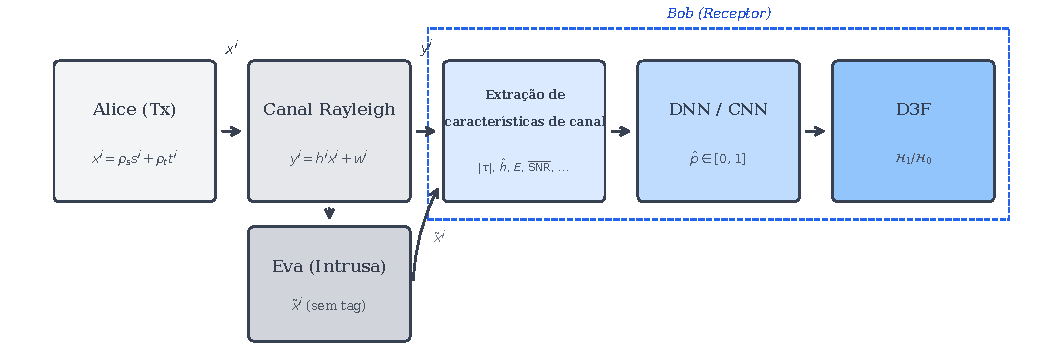
\includegraphics[width=\textwidth]{figures/fig_system_diagram}
  \caption{\label{fig:system}Diagrama do sistema de autenticação na camada física proposto. Alice transmite $x^i = \rho_s s^i + \rho_t t^i$, incorporando a sequência TAG caótica $t^i$. O canal Rayleigh introduz desvanecimento $h^i$ e ruído AWGN $w^i$, produzindo $y^i$ em Bob. O receptor extrai características de canal e as classifica por DNN ou 1D CNN com o framework D3F — gerando o escore $\hat{p} \in [0,1]$ que, comparado ao limiar $\tau^*(\alpha)$~\eqref{eq:d3f}, decide entre $\mathcal{H}_1$ (Alice autêntica) e $\mathcal{H}_0$ (intruso). Eva tenta se autenticar sem possuir a TAG legítima $t^i$.}
\end{figure*}


\section{Métodos Avaliados}\label{sec:methods}

Esta seção descreve todos os discriminadores investigados. A investigação segue uma progressão lógica motivada por duas perguntas em sequência:

\begin{enumerate}
  \item \textbf{Qual representação de entrada?} Sinal bruto $\mathbf{z}_{eq} \in \mathbb{R}^{1024}$ (a rede aprende tudo implicitamente) \emph{vs.} características escalares extraídas com motivação física.
  \item \textbf{Qual o conjunto mínimo de características?} Dadas as características físicas, qual subconjunto é necessário e suficiente para superar o correlador clássico?
\end{enumerate}

Para responder: (i)~1D CNN sobre $\mathbf{z}_{eq}$ testa o limite inferior de engenharia de características; (ii)~4-feat DNN com $\mathbf{f} = [|\tau|, \hat{h}, \overline{\text{SNR}}, E]$ é o ponto de partida física; (iii)~variações arquiteturais (CNN-4feat, CNN-2feat) separam efeito de características do efeito de topologia; (iv)~estudo de ablação de $\mathbf{f}$ identifica o núcleo mínimo.

\subsection{DNN com Quatro Características (4-feat DNN)}\label{sec:dnn4feat}

A DNN de quatro características é o ponto de partida natural: antes de saber qual o mínimo necessário, reunimos os quatro descritores mais informativos que a teoria de detecção sugere. A rede recebe $\mathbf{f} = [|\tau^i|,\, \hat{h},\, \widehat{\text{SNR}},\, E]$ e cada componente tem justificativa independente~\cite{ref_poor}:

\begin{itemize}
  \item \textbf{$|\tau^i|$} --- módulo do correlador casado~\eqref{eq:tau}: é a \emph{estatística suficiente} do teste de Neyman-Pearson ótimo para o modelo gaussiano de~\eqref{eq:dists}~\cite{ref_poor}. Equivale ao filtro casado com a tag, que maximiza o SNR de saída e concentra toda a informação discriminatória em um escalar~\cite{ref_proakis}. Fornecer $|\tau|$ explicitamente é a diferença fundamental em relação à 1D CNN: a rede \emph{não precisa} aprendê-lo implicitamente.

  \item \textbf{$\hat{h}$ e $\widehat{\text{SNR}}$} --- estimativas do canal: o limiar analítico $\tau_0^i = \sigma_{v^i}\,Q^{-1}(\alpha) \propto 1/\sqrt{\gamma^i}$ varia de pacote a pacote com $h^i$. Fornecer estimativas do ganho e da SNR permite à DNN aprender essa dependência --- comportamento análogo ao detector CFAR (\textit{Constant False Alarm Rate})~\cite{ref_poor}, que escala o limiar pelo nível de ruído corrente para manter $\alpha$ constante independentemente do canal.

  \item \textbf{$E = \|\mathbf{y}\|^2/L$} --- energia média do sinal recebido: sob $H_0$, $E \approx \sigma_w^2$; sob $H_1$, $E$ cresce com $\rho_t^2(h^i)^2\|\mathbf{t}^i\|^2/L$, provendo informação complementar.
\end{itemize}

A topologia adotada é:
\begin{equation}\label{eq:arch4feat}
\underbrace{[4]}_{\text{entrada}}\!\to\!\underbrace{\text{D}(256)\!\to\!\text{D}(128)\!\to\!\text{D}(64)}_{\text{ocultas}}\!\to\!\underbrace{[1]}_{\sigma(\cdot)},
\end{equation}
onde cada camada D$(n)$ inclui Batch Normalization, ReLU e Dropout ($p = 0{,}3$). O modelo tem ${\approx}\,44{.}000$ parâmetros treináveis. Para verificar se o desempenho provém das características ou da topologia, treinamos também a \textbf{DNN-1024}: mesma topologia Dense, mas recebendo $\mathbf{z}_{eq} \in \mathbb{R}^{1024}$ como entrada. Sem $|\tau|$ explícito, a DNN-1024 precisaria aprender o filtro casado implicitamente --- o que é inviável em baixo SNR.

\subsection{1D CNN com Sinal Residual Bruto ($\mathbf{z}_{eq}$)}\label{sec:cnn1d}

A 1D CNN~\cite{ref_liao,ref_oshea2017} processa diretamente o sinal residual $\mathbf{z}_{eq} \in \mathbb{R}^{1024}$, eliminando a necessidade de extração manual de características. A motivação teórica repousa na capacidade das redes convolucionais de explorar \emph{estrutura local} em sinais --- um princípio bem estabelecido em processamento de sinais e deep learning~\cite{ref_sainath2015,ref_oshea2017}. Ao contrário de camadas totalmente conectadas (Dense), que tratam todas as dimensões de entrada com igual importância, camadas convolucionais exploram três propriedades fundamentais: (i)~\textbf{localidade restrita}, onde cada neurônio conecta-se apenas a uma janela local (receptive field) do sinal; (ii)~\textbf{compartilhamento de pesos}, aplicando os mesmos filtros em posições diferentes ao longo do tempo; e (iii)~\textbf{pooling hierárquico}, que captura estrutura em múltiplas escalas temporais~\cite{ref_sainath2015}. Para sinais com correlações temporais ou frequenciais intrínsecos --- como $\mathbf{z}_{eq}$, que codifica a TAG caótica localmente correlacionada --- essas propriedades resultam em maior eficiência de aprendizado em relação a arquiteturas totalmente conectadas com o mesmo número de parâmetros~\cite{ref_oshea2017}.

A motivação prática é análoga à de um banco de filtros adaptativos: uma camada Conv1D com $c$ filtros de tamanho $k$ equivale a $c$ filtros FIR de ordem $k$ cujos coeficientes são otimizados por retropropagação~\cite{ref_proakis}.

\begin{equation}\label{eq:cnn1d}
\underbrace{[1024,1]}_{\mathbf{z}_{eq}}\!\to\!\text{Conv}_{32}^{15}\!\to\!\text{Conv}_{64}^{9}\!\to\!\text{Conv}_{128}^{5}\!\to\!\text{GAP}\!\to\!\text{D}(64)\!\to\![1],
\end{equation}
onde $\text{Conv}_{c}^{k}$ denota convolução 1D ($c$ filtros, kernel $k$) seguida de BN, ReLU e MaxPooling(4). O modelo tem ${\approx}\,69{.}000$ parâmetros.

\textbf{Por que esta arquitetura falha em baixo SNR?} A TAG tem energia $\rho_t^2 \approx 4{,}5\%$ da potência total. Sem acesso à tag de referência $\mathbf{t}^{\mathrm{ref}}$, a rede precisaria aprender o filtro casado implicitamente, o que exige que padrões da TAG sejam distinguíveis do ruído \emph{antes} de qualquer integração coerente. Em baixo SNR, a TAG está completamente encoberta pelo ruído amostra a amostra. Esta é uma limitação \emph{estrutural} --- não de capacidade da rede --- investigada em detalhe no segundo estudo de ablação (NN\_02c).

\subsection{CNN com Quatro Características (CNN-4feat)}\label{sec:cnn4feat}

Para isolar o efeito da \emph{arquitetura} do efeito das \emph{características}, treinamos uma CNN que aplica Conv1D sobre as mesmas quatro características $\mathbf{f}$ da 4-feat DNN:
\begin{equation}\label{eq:cnn4feat}
[4,1]\!\to\!\text{Conv}_{16}^{2}\!\to\!\text{Conv}_{32}^{2}\!\to\!\text{GAP}(32)\!\to\!\text{D}(16)\!\to\![1],
\end{equation}
com ${\approx}\,1{.}000$ parâmetros treináveis. Se CNN-4feat e 4-feat DNN atingirem desempenhos similares, isso valida o resultado central de D3F~\cite{ref_braca}: \emph{a topologia é irrelevante quando as características e a função de perda são adequadas.}

\subsection{Núcleo Mínimo: DNN e CNN com Duas Características}\label{sec:dnn2feat}

A rede neural densa recebe $\mathbf{f} = [|\tau^i|, \hat{h}^i]$, onde:
\begin{itemize}
  \item \textbf{$|\tau^i|$}: módulo do correlator casado~\eqref{eq:tau}, estatística suficiente para o teste NP ótimo sob modelo gaussiano~\eqref{eq:dists}~\cite{ref_poor}.
  \item \textbf{$\hat{h}^i$}: estimativa do ganho Rayleigh via mínimos quadrados. Seu papel é permitir à rede aprender limiares adaptativos em função do SNR instantâneo, implementando CFAR de forma implícita~\cite{ref_poor}.
\end{itemize}

A topologia é $[2] \to \text{D}(128) \to \text{D}(64) \to \text{D}(32) \to [1]$, onde cada camada inclui Batch Normalization, ReLU e Dropout ($p = 0{,}2$). O modelo tem ${\approx}\,10{.}000$ parâmetros treináveis. A simplicidade reforça o ponto teórico: dois escalares informativos são suficientes; arquitetura maior seria desnecessária.

\subsection{CNN-1D com Duas Características (CNN-2feat)}\label{sec:cnn2feat}

Para isolar o efeito de arquitetura, aplicamos Conv1D sobre a mesma entrada $\mathbf{f} = [|\tau^i|, \hat{h}^i]$:
\begin{equation}
[2,1] \to \text{Conv}_{8}^{1} \to \text{GAP} \to \text{D}(16) \to [1],
\end{equation}
onde Conv1D com kernel $k=1$ degrada-se a uma camada densa (sem convolução espacial relevante com apenas 2 features). O modelo tem ${\approx}\,200$ parâmetros. Qualquer diferença de desempenho entre DNN-2feat e CNN-2feat será atribuível apenas à variação arquitetural, validando o argumento de D3F que arquitetura é irrelevante se os dados satisfazem IID e BCE é usada.

\subsection{SVM Linear (referência não-neural)}\label{sec:svm}

Um SVM linear (perda \textit{hinge}, $\lambda = 10^{-4}$, 200 épocas, kernel linear) sobre $\mathbf{f} = [|\tau^i|, \hat{h}^i]$ maximiza a margem geométrica entre as classes em $\mathbb{R}^2$. Serve como referência clássica não-neural, confirmando que a discriminação é bem explicada por um hiperplano linear nos dois escalares fundamentais~\cite{ref_poor}.

\subsection{Protocolo de Treinamento}

Todos os classificadores neurais são treinados por minimização da BCE com o otimizador Adam~\cite{ref_adam} ($\eta_0 = 10^{-3}$, mini-lotes de 512 amostras), \textit{EarlyStopping} (paciência 20 épocas), \textit{ReduceLROnPlateau} (fator 0,5, paciência 10 épocas) e \textit{Dropout} ($p = 0{,}2$ em camadas convolucionais). A BCE incentiva escores calibrados — propriedade essencial para que a distribuição sob $H_0$ seja aproximadamente gaussiana e a extrapolação D3F via~\eqref{eq:d3f} seja válida.


\section{Dataset: Geração e Simulação}

\subsection{Modelo de Sinal e Parâmetros}

O dataset é gerado através de simulação Monte Carlo que reproduz fielmente as condições de canal e modulação. A transmissão autêntica (hipótese $H_1$) segue:
\begin{equation}\label{eq:sig_h1}
\mathbf{y}^i = h^i \left( \rho_s \mathbf{s}^i + \rho_t \mathbf{t}^i \right) + \mathbf{w}^i,
\end{equation}
onde $\rho_s = \sqrt{0{,}985} \approx 0{,}992$ é a amplitude da mensagem BPSK (1024 símbolos), $\rho_t = \sqrt{0{,}015 / 0{,}333} \approx 0{,}212$ é a amplitude da TAG (com normalização $\mathbb{E}[\mathbf{t}^2] \approx 1/3$ proveniente do mapa de tenda), $h^i$ é o ganho Rayleigh, e $\mathbf{w}^i \sim \mathcal{N}(\mathbf{0}, \sigma_w^2 \mathbf{I})$ é ruído AWGN. O ganho satisfaz $\mathbb{E}[(h^i)^2] = 1$, normalizando a potência de transmissão.

A transmissão fraudulenta (hipótese $H_0$) omite a TAG:
\begin{equation}\label{eq:sig_h0}
\mathbf{y}^i = h^i \rho_s \mathbf{s}^i + \mathbf{w}^i,
\end{equation}
refletindo que um atacante sem acesso à chave não pode reproduzir a sequência caótica. Bob estima o canal utilizando a mensagem conhecida e computa o correlator conforme Eq.~\ref{eq:tau}.

\subsection{Estratégia de Amostragem Estratificada}

O dataset é construído com 350.000 amostras balanceadas (175k por classe) distribuídas uniformemente em 6 bins de SNR: $[0,5)$, $[5,10)$, $\ldots$, $[25,30]$~dB. Sobreamostragem é aplicada em baixo SNR ($[0,10)$ dB): fator 1,5× para garantir que o modelo aprenda bem justamente onde a discriminação é mais difícil. Comprimento de mensagem varia em $[512, 1024]$ símbolos, zero-preenchido para 1024 em representação vetorial.

Cada amostra compreende:
\begin{itemize}
  \item $\mathbf{y}_{eq}^i = \mathbf{y}^i / h^i$ — sinal equalizado bruto (referência)
  \item $\mathbf{z}_{eq}^i = \mathbf{y}^i / h^i - \rho_s \mathbf{s}^i$ — resíduo após remoção da mensagem (entrada para CNN/DNN-1024)
  \item $\tau^i$ — correlator clássico (Xie 2021, Eq.~5)
  \item $h^i$, $\text{SNR}^i$ — metadados
  \item Rótulo: $y^i \in \{0, 1\}$
\end{itemize}

Diferença crítica: $\mathbf{z}_{eq}$ isola a TAG da mensagem conhecida. Sob $H_1$: $\mathbf{z}_{eq} = \rho_t \mathbf{t} + \mathbf{w}/h$ (TAG + ruído). Sob $H_0$: $\mathbf{z}_{eq} \approx \mathbf{w}/h$ (ruído puro, pois $(1-\rho_s) \approx 0{,}008 \ll 1$). Esta representação é essencial para redes que aprendem do sinal bruto.

\subsection{Particionamento e Normalização}

O dataset de 350k amostras é particionado respeitando estratificação por classe e SNR:
\begin{itemize}
  \item \textbf{Treino} (280k, 80\%): Otimização de parâmetros neurais
  \item \textbf{Validação} (35k, 10\%): Parada antecipada e ajuste de hiperparâmetros
  \item \textbf{Teste} (35k, 10\%): Avaliação final sem viés de treinamento
\end{itemize}

Características são normalizadas globalmente (z-score sobre o conjunto de treino) antes de alimentar as redes densas, garantindo convergência estável. Para a CNN 1D, normalização é aplicada por amostra (remover média e redimensionar cada vetor $\mathbf{z}_{eq}$ independentemente) para não remover informação de amplitude sensível ao SNR.


\section{Resultados e Discussão}\label{sec:results}

Esta seção consolida os resultados efetivamente executados nos notebooks NN\_02b, NN\_02c e NN\_07, todos sob o mesmo protocolo D3F com restrição $\alpha=10^{-7}$, canal Rayleigh e $L=1024$.

\subsection{Resultado Consolidado (NN\_07)}

O experimento unificado do NN\_07 confirmou a hierarquia de desempenho observada separadamente nos estudos de ablação. A Tabela~\ref{tab:comparacao} apresenta os principais métodos com resultados válidos no arquivo consolidado.

\begin{table}[htb]
\caption{\label{tab:comparacao}Comparação consolidada (NN\_07) --- $P_D$ (\%) sob $\alpha = 10^{-7}$, $L=1024$, Rayleigh.}
\begin{center}
\begin{tabular}{lrrrrrrr}\toprule
Método & 0~dB & 5~dB & 10~dB & 15~dB & 20~dB & 25~dB & 30~dB \\\midrule
Clássico~\cite{ref_xie}                         &  8{,}1 & 58{,}7 & 99{,}9 & 100{,}0 & 100{,}0 & 100{,}0 & 100{,}0 \\
V6 $[|\tau|,\hat{h}]$ (NN\_02b)               & 84{,}7 & 99{,}6 & 100{,}0 & 100{,}0 & 100{,}0 & 100{,}0 & 100{,}0 \\
V1 $[|\tau|,\hat{h},\overline{\text{SNR}},E]$ & 83{,}7 & 99{,}4 & 100{,}0 & 100{,}0 & 100{,}0 & 100{,}0 & 100{,}0 \\
z\_eq CNN (Var A, NN\_02c)                     &  0{,}4 &  0{,}1 &  0{,}0 &  86{,}2 & 100{,}0 & 100{,}0 & 100{,}0 \\
z\_eq + h (Var B, NN\_02c)                     &  0{,}2 &  0{,}1 &  0{,}0 &  88{,}0 & 100{,}0 & 100{,}0 & 100{,}0 \\
z\_eq + h + SNR (Var C, NN\_02c)               &  0{,}0 &  0{,}0 &  0{,}0 &  99{,}3 & 100{,}0 &  0{,}0 &  0{,}0 \\
z\_eq + $|\tau|$ (Var D, NN\_02c)              & \textbf{88{,}3} & \textbf{99{,}7} & 100{,}0 & 100{,}0 & 100{,}0 & 100{,}0 & 100{,}0 \\\bottomrule
\end{tabular}
\end{center}
\end{table}

Os resultados consolidados indicam que a melhor curva em baixo SNR no conjunto executado foi a Variante D do NN\_02c (z\_eq + $|\tau|$), com $P_D=88{,}3\%$ em 0 dB. O núcleo V6 do NN\_02b permanece altamente competitivo ($84{,}7\%$ em 0 dB), com vantagem de menor dimensionalidade e interpretação física mais direta. O resultado clássico permanece como referência de piso em 0 dB ($8{,}1\%$), aproximadamente uma ordem de magnitude abaixo das abordagens com aprendizagem e informação de canal.

\subsection{Ablação Tau (NN\_02b)}

O estudo de ablação com variantes tau confirma que a inclusão de $\hat{h}$ é o ganho crítico para o regime de baixo SNR. A Tabela~\ref{tab:feat_ablation} resume os resultados finais exportados no arquivo \texttt{nn02b\_ablation\_results.json}.

\begin{table}[htb]
\caption{\label{tab:feat_ablation}NN\_02b --- suficiência do núcleo mínimo $[|\tau|,\hat{h}]$. $P_D$ (\%) sob $\alpha=10^{-7}$, $L=1024$, Rayleigh.}
\begin{center}
{\footnotesize
\begin{tabular}{lrrrrrrr}\toprule
Variante & 0~dB & 5~dB & 10~dB & 15~dB & 20~dB & 25~dB & 30~dB \\\midrule
Clássico ($|\tau|$ analítico)                &  8{,}1 & 58{,}7 & 99{,}9 & 100{,}0 & 100{,}0 & 100{,}0 & 100{,}0 \\\midrule
V5: $|\tau|$                                  &  0{,}0 & 99{,}0 & 100{,}0 & 100{,}0 & 100{,}0 & 100{,}0 & 100{,}0 \\
\textbf{V6}: $[|\tau|,\hat{h}]$              & \textbf{84{,}7} & \textbf{99{,}6} & 100{,}0 & 100{,}0 & 100{,}0 & 100{,}0 & 100{,}0 \\
V7: $[|\tau|,\hat{h},\overline{\text{SNR}}]$ & 82{,}0 & 99{,}5 & 100{,}0 & 100{,}0 & 100{,}0 & 100{,}0 & 100{,}0 \\
V8: $[|\tau|,\hat{h},E]$                      & 81{,}6 & 99{,}5 & 100{,}0 & 100{,}0 & 100{,}0 & 100{,}0 & 100{,}0 \\
V1: $[|\tau|,\hat{h},\overline{\text{SNR}},E]$ & 83{,}7 & 99{,}4 & 100{,}0 & 100{,}0 & 100{,}0 & 100{,}0 & 100{,}0 \\\bottomrule
\end{tabular}
}
\end{center}
\end{table}

No conjunto NN\_02b, a transição V5$\to$V6 mostra o principal salto funcional: $P_D$ em 0 dB passa de $0{,}0\%$ para $84{,}7\%$. Essa mudança confirma que a estatística $|\tau|$ isolada não é suficiente sob fading severo sem informação instantânea de canal. A adição de SNR nominal (V7) e energia (V8) não melhora o núcleo V6 e, ao contrário, introduz pequenas perdas, coerentes com redundância de informação e aumento desnecessário de dimensionalidade.

\subsection{Ablação z\_eq (NN\_02c)}

O NN\_02c avaliou diretamente a suficiência do sinal residual de dimensão 1024. A Tabela~\ref{tab:zeq_ablation} sintetiza os resultados exportados em \texttt{nn02c\_ablation\_results.json}.

\begin{table}[htb]
\caption{\label{tab:zeq_ablation}NN\_02c --- variantes com $z_{eq}$ e entradas auxiliares. $P_D$ (\%) sob $\alpha=10^{-7}$, $L=1024$, Rayleigh.}
\begin{center}
{\footnotesize
\begin{tabular}{lrrrrrrr}\toprule
Variante & 0~dB & 5~dB & 10~dB & 15~dB & 20~dB & 25~dB & 30~dB \\\midrule
Clássico ($|\tau|$ analítico) & 8{,}1 & 58{,}7 & 99{,}9 & 100{,}0 & 100{,}0 & 100{,}0 & 100{,}0 \\\midrule
A: z\_eq somente             & 0{,}4 & 0{,}1 & 0{,}0 & 86{,}2 & 100{,}0 & 100{,}0 & 100{,}0 \\
B: z\_eq + h                 & 0{,}2 & 0{,}1 & 0{,}0 & 88{,}0 & 100{,}0 & 100{,}0 & 100{,}0 \\
C: z\_eq + h + SNR           & 0{,}0 & 0{,}0 & 0{,}0 & 99{,}3 & 100{,}0 & 0{,}0 & 0{,}0 \\
D: z\_eq + $|\tau|$          & \textbf{88{,}3} & \textbf{99{,}7} & 100{,}0 & 100{,}0 & 100{,}0 & 100{,}0 & 100{,}0 \\\bottomrule
\end{tabular}
}
\end{center}
\end{table}

As variantes A e B confirmam limitação estrutural de entrada baseada apenas em $z_{eq}$ no regime de baixo SNR, com desempenho praticamente nulo entre 0 e 10 dB. A Variante D, ao incorporar explicitamente $|\tau|$, recupera imediatamente o regime de alta detecção desde 0 dB, o que reforça o papel da estatística de correlação explícita como mecanismo de integração coerente. A Variante C apresentou comportamento inconsistente em 25 e 30 dB no arquivo exportado; por essa razão, sua interpretação deve ser tratada como evidência preliminar e sujeita a validação adicional.

\section{Conclusões}\label{sec:conclusions}

Os resultados executados em NN\_02b, NN\_02c e NN\_07 confirmam três conclusões centrais. A primeira é que a representação de entrada domina o desempenho em baixo SNR. Modelos que recebem estatísticas de correlação explícitas e informação instantânea de canal superam de forma consistente a referência clássica em 0 dB. A segunda é que o núcleo $[|\tau|,\hat{h}]$ permanece o melhor compromisso entre desempenho, interpretabilidade e simplicidade, atingindo $84{,}7\%$ de detecção em 0 dB com dimensionalidade mínima. A terceira é que variantes baseadas em $z_{eq}$ somente exibem limitação estrutural em baixo SNR, e a inclusão explícita de $|\tau|$ restaura desempenho elevado, como observado na Variante D do NN\_02c.

A consolidação no NN\_07 confirmou que os ganhos observados nos notebooks individuais não são artefatos locais de execução, mas refletem uma tendência estável do problema: integração coerente explícita e adaptação ao canal instantâneo são os dois fatores determinantes sob restrição ultraestrita de falso alarme ($\alpha=10^{-7}$). Esses resultados sustentam a formulação do detector orientado a dados no contexto de PLA com fading Rayleigh.

Como próximos passos, o estudo pode ser estendido para cenários veiculares não estacionários, com dinâmica temporal e canais Rician, mantendo o mesmo protocolo de comparação justa entre variantes de entrada e classes de classificador. Esse avanço permitirá separar, com maior precisão, o que decorre da física do canal e o que decorre da capacidade de modelagem da arquitetura.

\section*{Agradecimentos}
Os autores agradecem ao Departamento de Eletrônica e Sistemas da Universidade Federal de Pernambuco pelo apoio na realização deste trabalho.

\section*{Lista de Siglas}
{\small
\begin{tabular}{@{}p{1.9cm}p{5.9cm}@{}}
\textbf{1D CNN}    & \textit{One-Dimensional Convolutional Neural Network} \\
\textbf{AWGN}      & \textit{Additive White Gaussian Noise} \\
\textbf{BCE}       & \textit{Binary Cross-Entropy} (Entropia Cruzada Binária) \\
\textbf{BN}        & \textit{Batch Normalization} \\
\textbf{BPSK}      & \textit{Binary Phase Shift Keying} \\
\textbf{CFAR}      & \textit{Constant False Alarm Rate} (Taxa Constante de Falso Positivo) \\
\textbf{CNN}       & \textit{Convolutional Neural Network} \\
\textbf{CSI}       & \textit{Channel State Information} \\
\textbf{D3F}       & \textit{Data-Driven Detection Framework}~\cite{ref_braca} \\
\textbf{DNN}       & \textit{Deep Neural Network} \\
\textbf{GAP}       & \textit{Global Average Pooling} \\
\textbf{IoT}       & \textit{Internet of Things} \\
\textbf{LRT}       & \textit{Likelihood Ratio Test} \\
$\boldsymbol{P_D}$ & Probabilidade de Detecção \\
\textbf{PLA}       & \textit{Physical Layer Authentication} \\
\textbf{ReLU}      & \textit{Rectified Linear Unit} \\
\textbf{SNR}       & \textit{Signal-to-Noise Ratio} \\
\textbf{SVM}       & \textit{Support Vector Machine} \\
\textbf{TCL}       & Teorema Central do Limite \\
\end{tabular}
}

\begin{thebibliography}{99}

\bibitem{ref_sainath2015} T. N. Sainath, A. R. Mohamed, B. Kingsbury, e B. Ramabhadran, ``Convolutional, Recurrent, and Fully Connected Deep Neural Networks for Acoustic Modeling,'' em \textit{Proc.\ IEEE Int.\ Conf.\ Acoust.\ Speech Signal Process.\ (ICASSP)}, Vancouver, BC, Canadá, 2013, pp.~6645--6649.

\bibitem{ref_oshea2017} T. J. O'Shea e J. Hoydis, ``An Introduction to Deep Learning for the Physical Layer,'' \textit{IEEE Trans.\ Cogn.\ Commun.\ Netw.}, v.~3, n.~4, pp.~563--575, 2017.

\bibitem{ref_xie} H. Xie, W. Chen, e J. Ning, ``Security Model of Authentication at the Physical Layer and Performance Analysis over Fading Channels,'' \textit{IEEE Trans.\ Inf.\ Forensics Security}, v.~16, pp.~3945--3959, 2021.

\bibitem{ref_braca} P. Braca, S. Marano, V. Matta, e P. Willett, ``Statistical Hypothesis Testing Based on Machine Learning: Large Deviations Analysis,'' \textit{IEEE Open J.\ Signal Process.}, v.~3, pp.~464--484, 2022.

\bibitem{ref_liao} L. Liao, O. Wijesinghe, J. Perez-Ramirez, A. Bhatt, B. Imtiaz, e K. Ding, ``Deep Learning for Wireless Communications,'' \textit{Sensors}, v.~19, n.~11, p.~2440, 2019.

\bibitem{ref_joao} J. V. C. Evangelista, D. Moreno, D. P. B. Chaves e C. Pimentel, ``Tag Generation Using Chaotic Sequences for Physical-Layer Authentication,'' \textit{IEEE Access}, v.~11, pp.~73080--73087, 2023.

\bibitem{ref_yu} P. L. Yu, J. S. Baras, and B. M. Sadler, ``Physical-Layer Authentication,'' \textit{IEEE Trans.\ Inf.\ Forensics Security}, v.~3, n.~1, pp.~38--51, Mar.\ 2008.

\bibitem{ref_poor} H. V. Poor, \textit{An Introduction to Signal Detection and Estimation}, 2.~ed. Springer-Verlag, 1994.

\bibitem{ref_adam} D. P. Kingma e J. Ba, ``Adam: A Method for Stochastic Optimization,'' em \textit{Proc.\ Int.\ Conf.\ Learn.\ Represent.\ (ICLR)}, San Diego, CA, EUA, 2015.

\bibitem{ref_goodfellow} I. Goodfellow, Y. Bengio e A. Courville, \textit{Deep Learning}. MIT Press, 2016. Disponível em: \texttt{https://www.deeplearningbook.org}.

\bibitem{ref_proakis} J. G. Proakis e D. G. Manolakis, \textit{Digital Signal Processing: Principles, Algorithms, and Applications}, 4.~ed. Pearson Prentice Hall, 2007.

\bibitem{ref_3gpp} 3GPP, ``Study on Channel Model for Frequencies from 0.5 to 100 GHz,'' Technical Report TR 38.901, v17.0.0, 3rd Generation Partnership Project, 2022.

\bibitem{ref_shlezinger} N. Shlezinger, N. Farsad, Y.~C. Eldar e A.~J. Goldsmith, ``Model-Based Machine Learning for Communications,'' arXiv:2101.04726, 2021.

\bibitem{ref_veldhuis} R. Veldhuis e D. Zeng, ``On Neyman-Pearson Optimality of Binary Neural Net Classifiers,'' Tech.\ Rep., jun.\ 2021. DOI: 10.36227/techrxiv.14709930.v1.

\bibitem{ref_kay} S. M. Kay, \textit{Fundamentals of Statistical Signal Processing, Vol.~I: Estimation Theory}. Prentice Hall, 1993.

\bibitem{ref_raya} M. Raya e J.-P. Hubaux, ``Securing Vehicular Ad Hoc Networks,'' \textit{J. Comput. Secur.}, v.~15, n.~1, pp.~39--68, 2007.

\bibitem{ref_digham} F. F. Digham, M.-S. Alouini e M. K. Simon, ``On the Energy Detection of Unknown Signals Over Fading Channels,'' \textit{IEEE Trans.\ Commun.}, v.~55, n.~1, pp.~21--24, Jan.\ 2007.

\end{thebibliography}

\end{document}
